\lhead{Introduksjon}
\chapter{Innlending}
\section{Bakgrunn}
Rusta Vrak bilutleige er et lite firma basert i Førde og Jøster i Sogn og Fjordane. Utleie firmaet blir driftet av verkstedmesteren Stein Olav Erikstad, og målet er å kunne tilby utleie av greie og fult funksjonelle biler til en rimelig pris. Firmaet ble startet i 2013, og har i dag en flåte på over 20 biler. Rusta Vrak fungerer i dag som et sideprosjekt, men det har gode muligheter for vekst i fremtiden, men dersom et bilutleige firma ønsker å være kompetitivt, er det viktig å kunne tilby en digital form for tilgjengelighet på lik linje som de mer etablerte bedriftene. Derfor har Rusta Vrak Bilutleige uttryket ønske om å få en 


\section{Problemdefinisjon}
Rusta Vrak Bilutleie har i dag en nettside basert på tjenesten Blogspot [CITATION], som gjør at det er en enkel informasjonsside som oppgir informasjon om bilene, priser og kontaktinformasjon. Deretter må kunden ta kontakt enten vha. telefon eller epost for å foreta selve bestilling. Da firmaet blir driftet av én person som et sideprosjekt, kan det være vanskelig å alltid være tilgjengelig, og samtidig ha en oversikt over hvilke biler som er ledige til enhver tid. (ASD)

Dette kan bli forbedret ved å gjøre nettsiden mer interaktiv både for kunde og bedrift. 

\subsection{Oppgaven}
Lag en nettside for bilutleie firmaet Rusta Vrak Bilutleige. Denne nettsiden skal kunne benyttes av kunder for å finne hvilke biler som passer best for kundens formål, få en oversikt over når de spesifikke bilene er ledige for utleie, og foreta en reservasjon av valgt bil.

Nettsiden skal også kunne benyttes av firmaet for å få en oversikt over bilene som er for utleie, samt kunder som leier eller har leid bil. Det må være mulig å legge til, fjerne og redigere bilene for utleie forløpende.


\subsection{Krav} \label{kravliste1}
I samarbeid med firmaet utarbeidet vi noen krav over hva som er viktig å få med i nettsiden. Disse kan være både funksjonelle og ikke-funksjonelle.
\begin{description}
\item[Lett å bruke.]Nettsiden skal være enkel å bruke, og skal helst være så intuitiv som mulig. Det betyr at den ikke skal for komplisert i bruk.
\item[Skalere til alle skjermstørrelser.]Skalering mellom skjermstørrelser. Gjøre nettsiden like god å bruke på smartphone som på PCer.
\item[Selvstendig og Billig.]Firmaet er lite, og derfor skal nettsiden kunne være så selvstendig som mulig. Dvs. arbeid med drift og opprettholdning skal være minimal. Utover dette burde hosting av nettsiden også være rimelig.
\item[Håndere alle reservasjoner.]Nettsiden skal både fungere som et bestillingsverktøy for kunder, og som et verktøy for bedriften. Derfor skal brukere kunne benytte nettsiden for reservasjoner, og ansatt skal ha et administrasjons område hvor det er mulig å legge til nye bestillinger.
\item[Fordel å leie i lange perioder.]Det skal være en fordel å leie over lengre perioder. Systemet må ta hensyn til dette og det skal implementeres en funksjon for å kalkulere prisen.
\end{description}



\section{Problemløsning}
\subsection{Prosjekt Plan} \label{kravliste2}
Det første som ble gjort mot denne oppgaven var å lage en plan over alle funksjoner og arbeidsoppgaver som må med i det endelige produktet, og legge disse inn i kategorier basert på viktighet. Kategoriene går fra 1 til 5, og planen var å gå stegvis gjennom denne listen. 
 \begin{enumerate}
 
  \item \textbf{Oppsett og Installasjon}
  \begin{enumerate}
  	\item \textbf{Lokalt Utviklingsmiljø} - Installere Python, oppsett av virtualenv, Installere og integrere JetBrains PyCharm, installere Django.
  	\item \textbf{Lokal Database} - Installasjon og opprette kobling mellom Django prosjekt og lokal MySQL database.
  	\item \textbf{Google Cloud Platform} - Installering og oppsett av kobling mellom lokalt prosjekt og Google Cloud Platform. Dette inkluderer både hosting og database
  \end{enumerate}
  
  \item \textbf{Første Steg i Utviklingen}
  \begin{enumerate}
  	\item \textbf{Database Tabeller} - Planlegging og oppretting av database modeller og tabellene.
  	\item \textbf{Forside} - Enkel forside.
  	\item \textbf{Admin} - Mulighet til å legge til / slette biler fra opprettet database.
  	\item \textbf{Generere liste over biler fra database} - Basert på biltype.
  	\item \textbf{Bil Reservasjon} - Mulighet å legge inn er reservasjon av bil som går mellom to datoer.
  \end{enumerate}
  
  \item \textbf{Videreutvikling}
  \begin{enumerate} 
  	\item \textbf{Bilder} - Mulighet for å kunne vise bilde av bilene. Både som thumbnail og alternativt galleri.
	\item \textbf{Kalender} - Gjør det mulig for kunde å ha visuell oversikt når den spesifikke bilen er ledig for utleie. 
	\item \textbf{Epost Bekreftelse} - Send en email til kunde som bestiller. Denne skal inneholde informasjon om bestillingen.
	\item \textbf{Reservasjon Håndtering} - Legg til funksjonalitet som stopper en reservasjon fra å krasje med annen allerede eksisterende reservasjon.
	\item \textbf{Søkefunskjon} - Finne ledige biler på dato.
  \end{enumerate}
  
  \item \textbf{Ekstra Funksjonalitet}
	\begin{enumerate}
		\item \textbf{Pris Funksjon} - Det skal være en fordel å leie over lengre perioder. Derfor må en funksjon kunne dele ut riktig mengde rabatt over hvor mange dager som er i leieperioden. Videre skal denne kunne runde til nærmeste 5 for å slippe for mye småpenger.
		\item \textbf{PDF} - Mulighet å laste ned PDF med bestillingsdetaljer.
		\item \textbf{Filtrering av bil liste} - F.eks. kun biler som har automat. 
		\item \textbf{Konfigurering av Admin} - Søk bil på skiltnr., oversikt over alle reservasjoner og kunde informasjon.
	\end{enumerate}
  \item \textbf{Dersom tid}
  	\begin{enumerate}
  	\item \textbf{Google Calendar} - Legg til informasjon i en Google Calendar for enkel oversikt over når biler hentes og leveres.
  	\end{enumerate}
 
 \end{enumerate}
 
 
\subsection{Arbeidsmetode}
Utviklingen av dette prosjektet har benyttet en iterativ og inkrementell arbeidsmetode. Denne metoden går ut på å gjennomføre utviklingen stegvis, man begynner utviklingen med et skjelett, som man vil videre legge til litt funksjonalitet, og deretter komme tilbake og legge til mer på toppen av dette igjen. Ved å benytte en slik prosess, blir det mulig å utvikle flere områder på nettsiden samtidig uten at det nødvendigvis krasjer mellom de forskjellige funksjonene.

En iterativ metode gjør det mulig å splitte et større prosjekt i mindre, mer håndterlige biter. Utvikling av kode, planlegging og design blir gjennomført i gjenntatte sykluser \cite{method:iterative_fig}. Dermed kan man følge figur \ref{fig:iterative_development} for prosessen gjennom hele utviklingen.

 \begin{figure}[htbp]
	\centering
		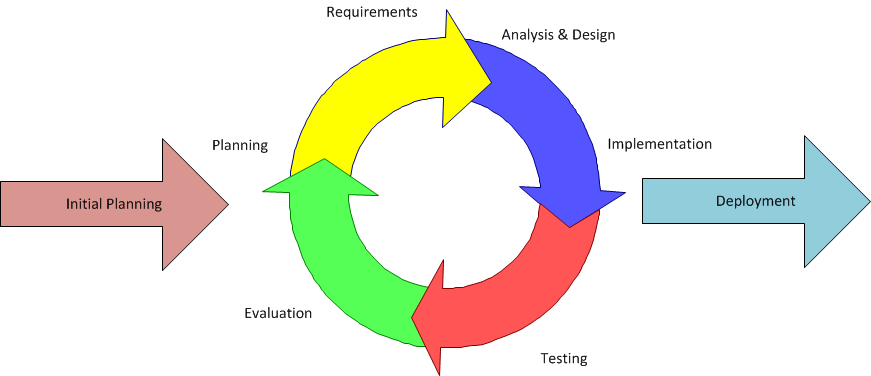
\includegraphics[scale=0.5]{Bilder/iterativ_utvikling.png}
	\caption[Iterativ Utviklings Diagram]{Oversikt over trinnene per syklus i iterativ utvikling \cite{iterative:development}. } %\ref{fig:iterative}
	\label{fig:iterative_development}
\end{figure}



\section{Litteratur Studie}
Det aller meste av studie mot denne oppgaven har foregått på internett. Dette inkluderer hovedsakelig bruk av dokumentasjonen til de forskjellige rammeverker og plattformer. Utover dette har det blitt benyttet noen bøker som har fungert som oppslagsverk gjennom hele prosessen.

\subsubsection*{Bøker}
\begin{itemize}
\item Code Complete 2. Edition (Steve McConnel)
\item Programming Google App Engine with Python (Dan Sanderson)
\item HTML and CSS Design and Build Websites (Jon Duckett)
\end{itemize}
\newpage